\documentclass[a4paper,12pt]{article}
\usepackage[a4paper,top=1.3cm,bottom=2cm,left=1.5cm,right=1.5cm,marginparwidth=0.75cm]{geometry}
\usepackage{cmap}
\usepackage{mathtext}
\usepackage[T2A]{fontenc}
\usepackage[utf8]{inputenc}
\usepackage[english,russian]{babel}
\usepackage{siunitx}

\usepackage{graphicx}

\usepackage{wrapfig}
\usepackage{tabularx}
\usepackage{multirow}

\usepackage{hyperref}
\usepackage[rgb]{xcolor}
\hypersetup{
colorlinks=true,urlcolor=blue
}
\usepackage{amsmath,amsfonts,amssymb,amsthm,mathtools}
\usepackage{icomma}
\mathtoolsset{showonlyrefs=false}
\usepackage{euscript}
\usepackage{mathrsfs}
\DeclareMathOperator{\sgn}{\mathop{sgn}}
\newcommand*{\hm}[1]{#1\nobreak\discretionary{}
{\hbox{$\mathsurround=0pt #1$}}{}}

%%% Заголовок
\author{Макаров Лев Евгеньевич}
\title{Лабораторная работа №1.2.5

Изучение экспериментальных погрешностей на примере физического маятника
}
\date{\today}

\begin{document}

\begin{titlepage}
	\begin{center}
		{\large МОСКОВСКИЙ ФИЗИКО-ТЕХНИЧЕСКИЙ ИНСТИТУТ (НАЦИОНАЛЬНЫЙ ИССЛЕДОВАТЕЛЬСКИЙ УНИВЕРСИТЕТ)}
	\end{center}
	\begin{center}
		{\large Физтех-школа фотоники, электроники и молекулярной физики}
	\end{center}
	
	
	\vspace{4.5cm}
	{\huge
		\begin{center}
			{\bf Отчёт о выполнении лабораторной работы 1.3.1 и 1.3.2}\\
			Определение моудля Юнга по измерениям растяжения проволоки и модуля сдвига при помощи крутильных колебаний
		\end{center}
	}
	\vspace{2cm}
	\begin{flushright}
		{\LARGE Автор:\\ Макаров Лев Евгеньевич \\
			\vspace{0.2cm}
			Б04-306}
	\end{flushright}
	\vspace{8cm}
	\begin{center}
		Долгопрудный 2023
	\end{center}
\end{titlepage}

\section{Введение}

\textbf{Цель работы:} 
\begin{enumerate}
	\item экспериментально получить зависимость между напряжением и деформацией одностороннего растяжения и по результатам определить модуль Юнга
    \item определение модулей кручения и сдвига для проволки по измерениям периодов крутильных колебаний подвешенного на ней маятника
\end{enumerate}

\textbf{В работе используются:} 
\begin{itemize}
    \item прибор Лермантова
    \item проволока из исследуемого материала
    \item зрительная трубка со шкалой
    \item набор грузов
    \item микрометр
    \item рулетка
    \item секундомер
    \item линйка
\end{itemize}
\medskip

\section{Теоретические сведения}

\subsection{Теория к разделу 1.3.1}
\label{thery-1-3-1}
Растяжение проволоки соответствует напряженному состоянию вдоль одной оси, которое описывается формулой:
\begin{equation}
    \frac{F}{S} = E \frac{\Delta l}{l}
    \label{lermantov}
\end{equation}
    Эту формулу можно переписать также в следующем виде:
    \begin{equation}
        F = k\Delta l,
    \end{equation}
    где $k = ES / l$ -- жесткость проволоки.
    Измерения производятся на установке Лермантова.
    Направим зрительную трубку на зеркальце.
    Выведем формулу для расчета растяжения длины проволоки по показаниям шкалы
    прибора (см. рис. 1).
    Так как мы считаем проволоку слабо растяжимой, справедлива оценка $\Delta l \ll r$, где
    $r$ -- длина рычага. С учетом этого, угол наклона зеркальца к горизонтали можно
    найти как $\alpha = \Delta l/r$. С другой стороны, из соображений геометрической оптики
    угол $\alpha$ можно найти как угол между продолжениями соответствующих лучей:
    \begin{equation}
        \alpha = \frac{n}{2h},
    \end{equation}
    где $n$ -- показания шкалы, $h$ -- расстояние от шкалы до
    зеркальца.
    \par Таким образом, удлинение проволоки можно выразить как:
    \begin{equation}
        \Delta l = n\frac{r}{2h}
        \label{dlina}
    \end{equation}

    Отсюда формулу (1) можно переписать как
    \begin{equation}
        F = \frac{ESr}{2lh}n
    \end{equation}

\subsection{Теория к разделу 1.3.2}

При закручивании цилиндрических стержней круглого сечения распределение деформаций
 и напряжений одинаково по длине стержня только вдали от мест, где прикладываются закручивающие моменты.
Для этих областей можно считать, что каждое поперечное сечение поворачивается поворачивается как жествкое,
то есть частички материала не сходят с радиальных линий, на которых они были в начале, и все
эти линии поворачиваются на один и тот же угол. Такое напряженное состояние назвается чистым кручением.\\

При такой деформации любая прямая линия, проведенная до закручивания цилиндра почастицам материала и параллельная оси симметрии,
при закручивании превращается в спираль(винтовую линию). \\

Покажем, что касательное напряжение напряжение в поперечном сечении увеличивается пропорцианально
 расстоянию до оси вращения.
Рассмотрим в цилиндре колечко бесконечно малой толщиной $dr$ и высоты $dl$. При закручивании верхнее колечко поворачивается относительно 
нижнего на угол $d\varphi$, а образующая наклоняется на угол $\alpha$. Тогда при малы углах справедливо соотношение:
\begin{equation}
    \alpha dl= r d\varphi 
\end{equation}

Касательное наряжение $\tau $ связано с углом $\alpha$ линейной зависимостью через модуль сдвига $G$,
 и следовательно растет с увеличением расстоянием от оси:
\begin{equation}
    \tau = G\cdot \alpha =Gr\frac{d\varphi}{dl} 
\end{equation}

Эти касательные напряжения создают момент сил относительно оси цилиндра:

\begin{equation}
    dM=2\pi r dr \cdot r\cdot \tau  
\end{equation}

Интегрируя это выражение по всем колечкам от оси цилиндра до его радиуса R находим суммарный
момент сил:
\begin{equation}
    M = \frac{\pi G R^{4}}{2} \frac{d \varphi }{d l} 
\end{equation}

Так как момент сил не меняется по длине цилиндра. Тогда для связи приложенного
момента сил $M$ и угла поворота $\varphi$ поперечных сечений цилиндра имеем:
\begin{equation}
    M=\frac{\pi R^{4}G}{2l}\varphi=f \varphi
\end{equation}
Где $f$ - модуль кручения связанный с модулем сдвига $G$ соотношением:
\begin{equation}\label{sdvig}
    G=\frac{2l}{\pi R^{4}}f
\end{equation}

В системе можно возбудить крутильные колебания. Вращение стержня с закрепленными
на нем грузиками вокрунг вертикальной оси проиходит под действием упругого момента $M$.
С учетом выражения для момента $M$ получим, что это вращение описывается уравнением колебаний:
\begin{equation}
    I\frac{d^2 \varphi }{d t^2} + f \varphi =0
\end{equation}
Следовательно период кoлебаний системы связан с расстоянием $l_c$ от оси вращения до грузов и
моментом инерции стержня $I_0$ следующим образом:
\begin{equation}\label{t-2-of-l-2}
    T^2=\frac{4 \pi^2 I}{f}=\frac{4 \pi^2 I_0}{f} + \frac{4 \pi^2 (m_1+m_2)}{f}l_c^2
\end{equation}
Эти зависимости были получены для незатухающих колебаний. Поэтому для их применения необходимо убедиться,
что в рассматриваемой системе диссипативными силами можно пренебречь. Для этого стоит убедиться, что период колебаний
не зависит от начальной амплитуды и что амплитуда уменшьется не более чем в 2 раза после около 10 колебаний.

\section{Оборудование и экспериментальные погрешности}

\textbf{Секундомер:} $\sigma_s = \pm 0,03$ с \\ 
\textbf{Штангенциркуль:} $\sigma_\text{шт} = \pm 0,005$ см \\
\textbf{Линейка:} $\sigma_\text{шт} = \pm 1$ мм \\
\textbf{Измерительная шкала:} $\sigma_\text{шт} = \pm 0,1$ см \\
\textbf{Электронные весы ВЛТЭ-5100:} $\sigma_m = \pm 0,3$ г \\


\section{Результаты измерений и обработка данных работы 1.3.1}

\subsection{Определение площади поперечного сечения проволоки}

Площадь поперечного сечения проволоки не измерялась напрямую, а принята равной $d_\text{пр} = (0,46 \pm 0,01) \text{ мм}$.

Площадь поперечного сечения проволоки вычисляется по формуле: $S = \frac{\pi d_\text{пр}^2}{4} = 0,166 \text{ мм}^2$

Погрешность вычисления площади поперечного ыечения можно вычислить по формуле: $\sigma_S = \frac{\pi d_\text{пр}}{2} \sigma_d = 0,007 \text{ мм}^2$

\subsection{Измерение длины проволоки}

Длина проволоки измерялась после выполнения всех остальных измерений, чтобы не сбить настройки установки перед началом опыта. Длина проволоки $l = (176,2 \pm 0,1) \text{ см}$

\subsection{Вывод формулы удлинения проволоки}

Формула удлинения прволоки через чимло делений по шкале \eqref{dlina} была выведена в разделе \ref{thery-1-3-1}.

\subsection{Проверка максимальной нагрузки}

Проверим максимальную нагрузку на проволоку. Разрушающее напряжение примем за $T_\text{р} = 900 \frac{\text{Н}}{\text{мм}^2}$, рабочее напряжение не должно превышать $30 \%$ от $T_\text{р}$. Для проверки правильности этой оценки будем добавлять нагрузку постепенно, после чего убирать и сверять положение шкалы без дополнительной нагрузки. Повторим этот процесс для всего набора грузов. В процессе значение шкалы без дополнительной нагрузки колебалось в диапазоне от $21,9$ до $22,1$ см, что в пределах погрешности относительно начального положения в $22$ см. Из чего можно сделать вывод о правильности сделанной оценки.

\subsection{Зависимость удлиннения проволоки от массы}

Для получения зависимости удлиннения проволоки от массы будем постепенно добавлять грузы и замерять показвния шкалы для каждого добавленного груза. Результаты измерений запишем в таблицу \ref{udlin-uvel}. После чего будем удирать грузы по одному и снимать показания шкалы, результаты измерений запишем в таблицу \ref{udlin-umen}. Так же для каждого измерения посчитаем удлиннение проволоки по формуле \eqref{dlina}.

\begin{table}[!ht]
    \centering
    \begin{tabular}{|l|l|l|l|l|l|l|l|}
    \hline
        $N$ & $m_\text{общ}$, г & $m_\text{доб}$, г & $n$ & $\sigma_m$, г & $\sigma_n$ & $\Delta_l$, мм & $\sigma_{\Delta_l}$, мм \\ \hline
        0 & 0,0 & 0,0 & 21,9 & 0,3 & 0,1 & 1,15 & 0,08 \\ \hline
        1 & 246,1 & 246,1 & 25,1 & 0,6 & 0,1 & 1,32 & 0,09 \\ \hline
        2 & 491,7 & 245,6 & 27,8 & 0,9 & 0,1 & 1,46 & 0,10 \\ \hline
        3 & 737,0 & 245,3 & 30,5 & 1,2 & 0,1 & 1,60 & 0,11 \\ \hline
        4 & 982,5 & 245,5 & 33,2 & 1,5 & 0,1 & 1,74 & 0,12 \\ \hline
        5 & 1228,1 & 245,6 & 35,7 & 1,8 & 0,1 & 1,87 & 0,12 \\ \hline
        6 & 1472,5 & 244,4 & 38,3 & 2,1 & 0,1 & 2,01 & 0,13 \\ \hline
        7 & 1717,8 & 245,3 & 40,7 & 2,4 & 0,1 & 2,13 & 0,14 \\ \hline
        8 & 1963,4 & 245,6 & 43,3 & 2,7 & 0,1 & 2,27 & 0,15 \\ \hline
        9 & 2208,9 & 245,5 & 45,7 & 3,0 & 0,1 & 2,40 & 0,16 \\ \hline
        10 & 2454,5 & 245,6 & 48,4 & 3,3 & 0,1 & 2,54 & 0,17 \\ \hline
        11 & 2700,3 & 245,8 & 49,0 & 3,6 & 0,1 & 2,57 & 0,17 \\ \hline
    \end{tabular}\caption{\textit{Зависимость удлиннения от добавочной массы при увелечении массы}}\label{udlin-uvel}
\end{table}

\begin{table}[!ht]
    \centering
    \begin{tabular}{|l|l|l|l|l|l|l|l|}
    \hline
        $N$ & $m_\text{общ}$, г & $m_\text{убав}$, г & $n$ & $\sigma_m$, г & $\sigma_n$ & $\Delta_l$, мм & $\sigma_{\Delta_l}$, мм \\ \hline
        12 & 2700,3 & 0,0 & 49,0 & 3,6 & 0,1 & 2,57 & 0,17 \\ \hline
        11 & 2454,5 & 245,8 & 48,5 & 3,3 & 0,1 & 2,54 & 0,17 \\ \hline
        10 & 2208,9 & 245,6 & 46,2 & 3,0 & 0,1 & 2,42 & 0,16 \\ \hline
        9 & 1963,4 & 245,5 & 43,5 & 2,7 & 0,1 & 2,28 & 0,15 \\ \hline
        8 & 1717,8 & 245,6 & 41,0 & 2,4 & 0,1 & 2,15 & 0,14 \\ \hline
        7 & 1472,5 & 245,3 & 38,4 & 2,1 & 0,1 & 2,01 & 0,13 \\ \hline
        6 & 1228,1 & 244,4 & 35,9 & 1,8 & 0,1 & 1,88 & 0,13 \\ \hline
        5 & 982,5 & 245,6 & 33,2 & 1,5 & 0,1 & 1,74 & 0,12 \\ \hline
        4 & 737,0 & 245,5 & 30,7 & 1,2 & 0,1 & 1,61 & 0,11 \\ \hline
        3 & 491,7 & 245,3 & 28,0 & 0,9 & 0,1 & 1,47 & 0,10 \\ \hline
        2 & 246,1 & 245,6 & 25,2 & 0,6 & 0,1 & 1,32 & 0,09 \\ \hline
        1 & 0,0 & 246,1 & 22,3 & 0,3 & 0,1 & 1,17 & 0,08 \\ \hline
    \end{tabular}\caption{\textit{Зависимость удлиннения от добавочной массы при ууменьшении массы}}\label{udlin-umen}
\end{table}

Погрешность $\Delta_l$ для каждого значения рассчитаем по формуле \eqref{error-delta-l}.

\begin{equation}\label{error-delta-l}
    \sigma_{\Delta_l} = \sqrt{
    \left( \frac{d \Delta_l}{dn} \right) ^ 2 \sigma_{n}^2 + 
    \left( \frac{d \Delta_l}{dr} \right) ^ 2 \sigma_{r}^2 + 
    \left( \frac{d \Delta_l}{dh} \right) ^ 2 \sigma_{h}^2
    }
\end{equation}

\subsection{График зависимости удлинения от нагрузки}

Построим график зависимости удлинения проволоки $\Delta_l$ от нагрузки $P$. Для аппроксимации прямой возпользуемся МНК, где $u = \Delta_l$, а $v = P$. Так как зависимость должна быть прямой, получаем для двух прямых $k$ и $b$ рассчитываются по формулам:

\begin{equation}
    k = \frac{\langle uv\rangle - \langle u \rangle \langle v \rangle}{\langle v^2 \rangle - \langle v \rangle^2}
\end{equation}

\begin{equation}
    b = \langle u \rangle - k\langle v \rangle
\end{equation}

Погрешности для $k$ и $b$ рассчитываются по формулам:

\begin{equation}
    \sigma_k = \frac{1}{\sqrt{7}} \sqrt{\frac{\langle u^2 \rangle - \langle u \rangle^2}{\langle v^2 \rangle - \langle v \rangle^2} - k^2}
\end{equation}

\begin{equation}
    \sigma_b = \sigma_k\sqrt{\langle v^2 \rangle - \langle v \rangle^2}
\end{equation}

Отсюда получаем для добавления: $k_\text{доб} = (0,055 \pm 0,001) \ \frac{\text{мм}}{\text{Н}}$, $b_\text{доб} = (0,923 \pm 0,009) \text{ мм}$. Для убавления массы: $k_\text{убав} = (0,055 \pm 0,001) \ \frac{\text{мм}}{\text{Н}}$, $b_\text{убав} = (0,934 \pm 0,009) \text{ мм}$. График зависимости для добавления массы изображен на рис. \ref{adding-wheight}, график для убавления массы изображен на рис. \ref{removing-wheight}. График, на котором изображены обе зависимости, изображен на рис. \ref{graph-combined}.

\subsection{Определение модуля Юнга}

По наклону прямой определим определим жёсткость проволоки, а по ней модуль Юнга. Значение наклона прямой $k = (0,055 \pm 0,001) \ \frac{\text{мм}}{\text{Н}}$. Жёсткость пружины $K = \frac{1}{k} = 18220 \ \frac{\text{Н}}{\text{м}}$. Погрешность $\sigma_K = \frac{\sigma_k}{k^2} = 348 \ \frac{\text{Н}}{\text{м}}$.

Модуль Юнга $E$ можно вычислить по формуле:

\begin{equation}
    E = \frac{K l}{S} = 193 \text{ ГПа}
\end{equation}

Погрешность вычисления модуля Юнга можно вычислить по формуле:

\begin{equation}
    \sigma_E = \sqrt{
    \left( \frac{dE}{dK} \right)^2 \sigma_{K}^2 +
    \left( \frac{dE}{dl} \right)^2 \sigma_{l}^2 +
    \left( \frac{dE}{dS} \right)^2 \sigma_{S}^2
    } \approx 9 \text{ ГПа}
\end{equation}

\subsection{Определение материала проволоки}

Согласно справочным данным, полученное значение для модуля Юнга $E = (193 \pm 9)$ ГПа лежащее в интервале от 190 до 200 ГПа соответствует железу. Отсюда можно сделать вывод, что скорее всего проволока изготовлена из железа.

\section{Результаты измерений и обработка данных работы 1.3.2}

\subsection{Установление допустимых амплитуд отклонения}


\subsection{Проворка применимости установки}

Для того, чтобы установку можно было использовать, необходимо чтобы после десяти колебаний с амплитудой из установленного диапазона затухание было менее, чем в два раза. Так как это выполняется, то колебания можно считать гармоническими, а значит можно пренебречь затуханием во время работы.

\subsection{Измерение периодов колебаний}

Перед началом измерений измерим параметры цилиндров и запишем их в таблицу \ref{cilinders}. Из этих данных можно рассчитать моменты инерции каждого из цилиндров относительной осей, проходящих через центр масс каждого параллельно стержню. Результаты вычисления моментов инерции тоже запишем в таблицу. Момент инерции цилиндра через данную ось вычисляется по формуле:

\begin{equation}
    I = \frac{mH^2}{12} + \frac{md^2}{16}
\end{equation}

Погрешность момента инерции можно рассчитать по формуле:

\begin{equation}
    \sigma_I = \sqrt{
    \left( \frac{dI}{dm} \right)^2 \sigma_{m}^2 +
    \left( \frac{dI}{dh} \right)^2 \sigma_{h}^2 +
    \left( \frac{dI}{dd} \right)^2 \sigma_{d}^2
    }
\end{equation}

Вычислим погрешность измерения моментов инерции цилтиндров и запишем в таблицу \ref{cilinders}.

\begin{table}[!ht]
    \centering
    \begin{tabular}{|l|l|l|}
    \hline
        \textbf{хар-ка} & \textbf{цилиндр 1} & \textbf{цилиндр 2} \\ \hline
        $m$, г & 204,1 & 202,5 \\ \hline
        $h$, см & 4,02 & 4,05 \\ \hline
        $d$, см & 4,88 & 4,83 \\ \hline
        $I$, $\text{г} \cdot \text{м}^2$ & 3,065 & 2,980 \\ \hline
        $\sigma_I$, $\text{г} \cdot \text{м}^2$ & 0,005 & 0,004 \\ \hline
    \end{tabular}\caption{\textit{Характеристики цилиндров на установке}}\label{cilinders}
\end{table}



Будем утанавливать грузы на одинаковом расстоянии от стержня до центров масс грузов $l_c$ и два раза измерять период десяти колебаний. Повторим это для 17 различных значений $l_c$. Результаты измерений запишем в таблицу \ref{period-17}.

\begin{table}[!ht]
    \centering
    \begin{tabular}{|l|l|l|l|l|l|}
    \hline
        N & l, см & L\_C & T\_1, с & T\_2, с & t, c \\ \hline
        1 & 0,00 & 2,02 & 16,16 & 16,13 & 1,615 \\ \hline
        2 & 1,00 & 3,02 & 17,43 & 17,43 & 1,743 \\ \hline
        3 & 2,00 & 4,02 & 19,35 & 19,34 & 1,935 \\ \hline
        4 & 3,00 & 5,02 & 20,68 & 20,69 & 2,069 \\ \hline
        5 & 4,00 & 6,02 & 22,91 & 22,91 & 2,291 \\ \hline
        6 & 5,00 & 7,02 & 24,53 & 24,52 & 2,453 \\ \hline
        7 & 6,00 & 8,02 & 26,6 & 26,58 & 2,659 \\ \hline
        8 & 7,00 & 9,02 & 29,01 & 29,01 & 2,901 \\ \hline
        9 & 8,00 & 10,02 & 31,72 & 31,72 & 3,172 \\ \hline
        10 & 9,00 & 11,02 & 33,6 & 33,61 & 3,361 \\ \hline
        11 & 10,00 & 12,02 & 36,38 & 36,39 & 3,639 \\ \hline
        12 & 11,00 & 13,02 & 38,87 & 38,88 & 3,888 \\ \hline
        13 & 12,00 & 14,02 & 41,4 & 41,41 & 4,141 \\ \hline
        14 & 13,00 & 15,02 & 43,76 & 43,76 & 4,376 \\ \hline
        15 & 14,00 & 16,02 & 46,3 & 46,3 & 4,630 \\ \hline
        16 & 15,00 & 17,02 & 48,79 & 48,79 & 4,879 \\ \hline
        17 & 16,00 & 18,02 & 51,37 & 51,36 & 5,137 \\ \hline
    \end{tabular}\caption{\textit{Результаты измерения периодов колебаний}}\label{period-17}
\end{table}

Согласно соотношению \eqref{t-2-of-l-2} $t^2$ должно прямо зависить от $l_c^2$. Для аппроксимации наилучшей прямой этой зависимости воспользуемся МНК, где $u = t^2$, а $v = l_c^2$. Так как зависимость должна быть прямой, получаем для двух прямых $k$ и $b$ рассчитываются по формулам:

\begin{equation}
    k = \frac{\langle uv\rangle - \langle u \rangle \langle v \rangle}{\langle v^2 \rangle - \langle v \rangle^2} \approx 0,0741 \ \frac{\text{с}^2}{\text{см}^2}
\end{equation}

\begin{equation}
    b = \langle u \rangle - k\langle v \rangle \approx 2,44 \ \text{с}^2
\end{equation}

Погрешности для $k$ и $b$ рассчитываются по формулам:

\begin{equation}
    \sigma_k = \frac{1}{\sqrt{17}} \sqrt{\frac{\langle u^2 \rangle - \langle u \rangle^2}{\langle v^2 \rangle - \langle v \rangle^2} - k^2} \approx 0,0003 \ \frac{\text{с}^2}{\text{см}^2}
\end{equation}

\begin{equation}
    \sigma_b = \sigma_k\sqrt{\langle v^2 \rangle - \langle v \rangle^2} \approx 0,03 \ \text{с}^2
\end{equation}

График зависимости $t^2$ от $l_c^2$ изображён на расунке \ref{graph}. Согласно формуле \eqref{t-2-of-l-2} коэффициент наклона прямой равен:

\begin{equation}
    k = \frac{4 \pi^2 (m_1 + m_2)}{f} \ \implies \ f = \frac{4 \pi^2 (m_1 + m_2)}{k} \approx 0,02167 \text{ Н} \cdot \text{м}
\end{equation}

Погрешность вычисления модуля кручения можно вычислить по формуле:

\begin{equation}
    \sigma_f = \sqrt{
    \left( \frac{df}{dm_1} \right)^2 \sigma_{m_1}^2 +
    \left( \frac{df}{dm_2} \right)^2 \sigma_{m_2}^2 +
    \left( \frac{df}{dk} \right)^2 \sigma_{k}^2
    } \approx 0,00008 \text{ Н} \cdot \text{м}
\end{equation}

\subsection{Определение модуля сдвига}

Измерим диаметр проволоки с помощью штангенциркуля в 5 различных местах и результаты измерений запишем в таблицу \ref{diameter}.

\begin{table}[!ht]
    \centering
    \begin{tabular}{|l|l|l|l|l|l|}
    \hline
        n & 1 & 2 & 3 & 4 & 5 \\ \hline
        d, мм & 1,560 & 1,570 & 1,560 & 1,590 & 1,560 \\ \hline
    \end{tabular}\caption{\textit{Результаты измерения диампетра проволоки}}\label{diameter}
\end{table}

Тогда $d_\text{пр} = \frac{\sum d}{n} = 1,568$ мм, погрешность измерения соответственно равна: $\sigma_{d_\text{пр}} = \frac{\sigma_\text{шт}}{n} = 0,001$ мм. Длина проволоки известна и равна: $L = (1730 \pm 2) \text{ мм}$.

Воспользовавшись формулой \eqref{sdvig} вычислим модуль сдвига для проволоки: $G = 63,2 \text{ ГПа}$

Погрешность вычисления модуля сдвига $\sigma_G$ можно вычислить по формуле:

\begin{equation}
    \sigma_G = \sqrt{
    \left( \frac{dG}{dL} \right)^2 \sigma_{L}^2 +
    \left( \frac{dG}{df} \right)^2 \sigma_{f}^2 +
    \left( \frac{dG}{dd_\text{пр}} \right)^2 \sigma_{d_\text{пр}}^2
    } \approx 0,3 \text{ ГПа}
\end{equation}

Тогда $G = (63,2 \pm 0,3) \text{ ГПа}$. Так как материал проволоки известен -- сталь, то можно сравнить полученное значение для модуля сдвига с табличными значениями. Они варьируются от 45 до 90 ГПа, что не противоречит экспериментальным данным.

\section{Обсуждение результатов и выводы}

\subsection{Работа 1.3.1}

В ходе работы была получена зависимость между напряжением и деформацией одностороннего растяжения проволоки. По результатам был определён модуль Юнга $(193 \pm 9) \text{ ГПа}$ для проволоки, что соовтетствует железу.

\subsection{работа 1.3.2}

В ходк работы было получено значение модуля кручения $(0,02167 \pm 0,00008) \text{ Н} \cdot \text{м}$ и сдвига $(63,2 \pm 0,3) \text{ ГПа}$ для данной проволоки, что соответствует значениям данных величин для стали.

\newpage

\begin{figure}[h!]
    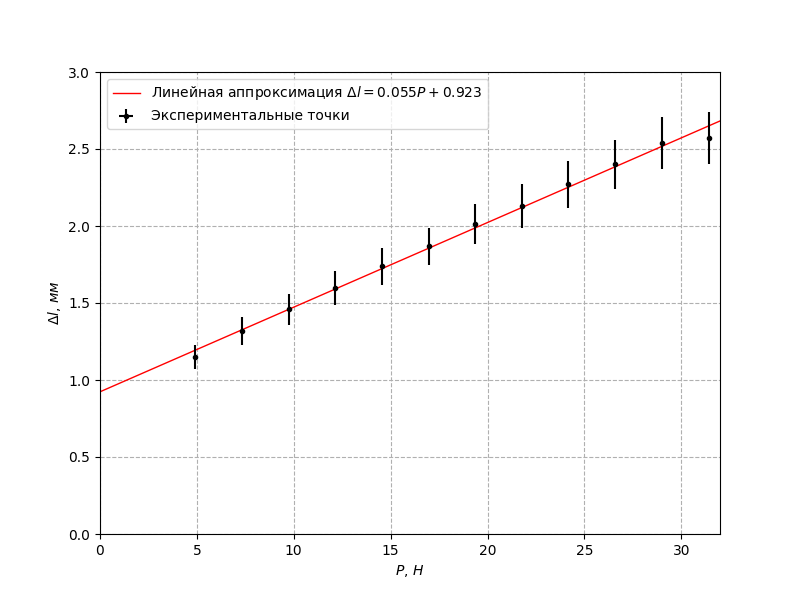
\includegraphics[width=1\textwidth]{adding-wheight.png}
    \caption{\textit{График зависимости $\Delta_l$ от $P$ при увелечении массы}}
    \label{adding-wheight}
\end{figure}

\begin{figure}[h!]
    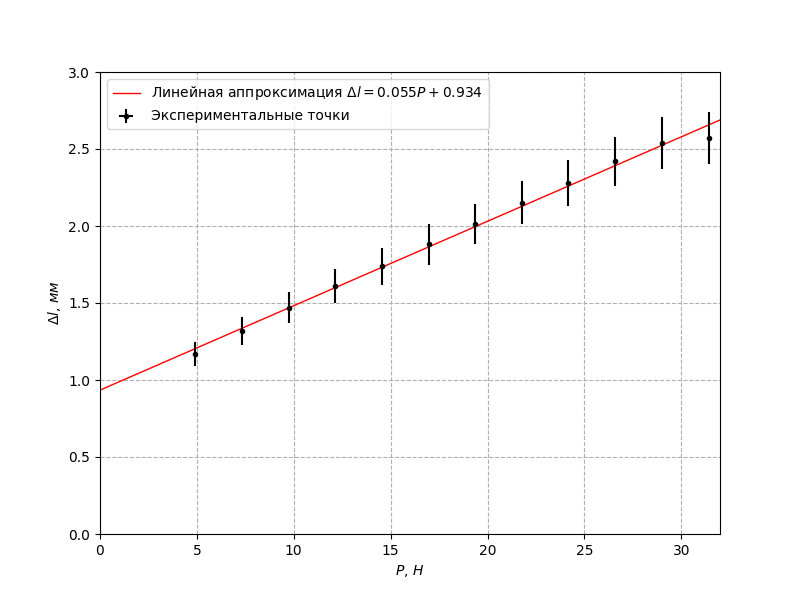
\includegraphics[width=1\textwidth]{removing-wheight.png}
    \caption{\textit{График зависимости $\Delta_l$ от $P$ при уменьшении массы}}
    \label{removing-wheight}
\end{figure}

\begin{figure}[h!]
    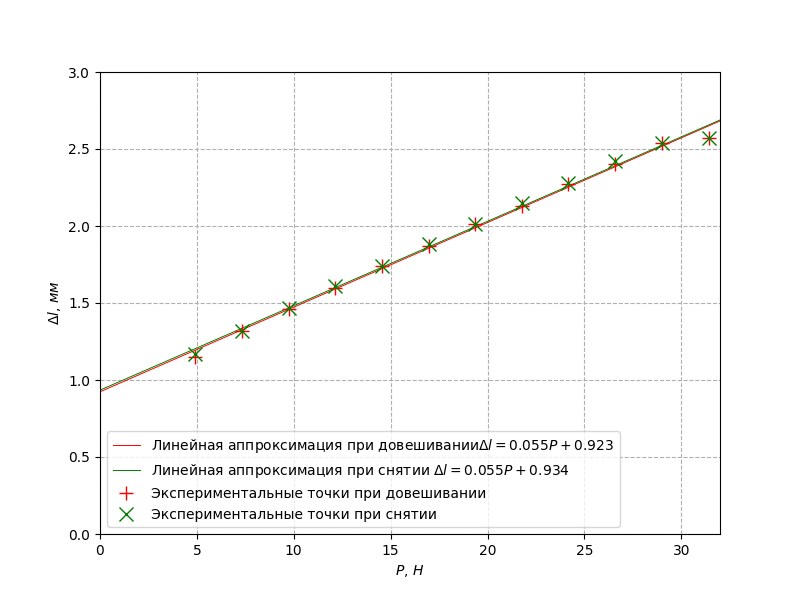
\includegraphics[width=1\textwidth]{graph-combined.png}
    \caption{\textit{График зависимости $\Delta_l$ от $P$ в обоих случаях}}
    \label{graph-combined}
\end{figure}

\begin{figure}[h!]
    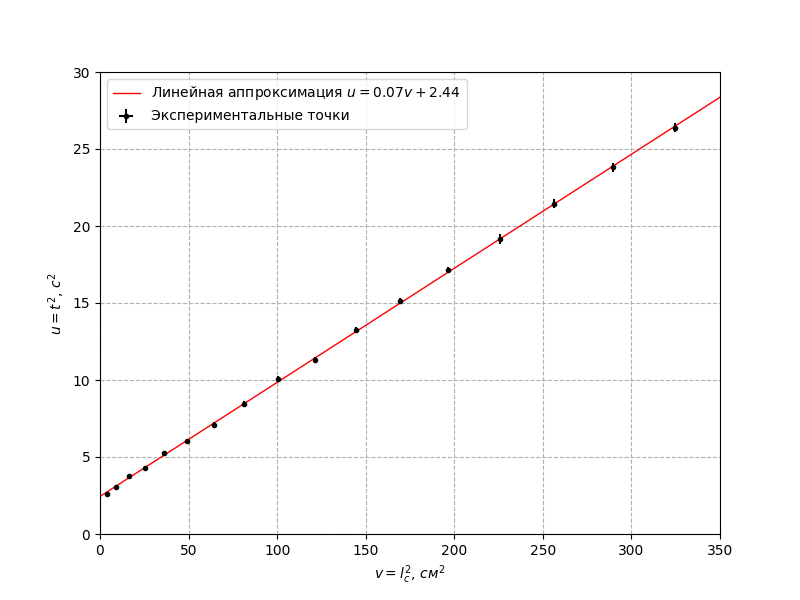
\includegraphics[width=1\textwidth]{graph.png}
    \caption{\textit{График зависимости $t^2$ от $l_c^2$}}
    \label{graph}
\end{figure}

\end{document}